\chapter{Algoritmos voraces}\label{voraces}

\section{Enunciado}\label{voraces-enunciado}

Sea $G$ un grafo no dirigido conexo.
$G$ es un grafo de Euler si, y sólo si, todo los vértices de $G$ tienen grado par.
Recordemos que el grado de un vértice es el número de aristas que empiezan (o terminan, según se mire) en él.
Un camino de Euler es un camino que no repite aristas y en el que aparecen todos las aristas del grafo.
Un circuito de Euler es un ciclo (empieza y termina en el mismo vértice) que, además, es un camino de Euler.
Sabiendo esto, diseñe un algoritmo \textit{Greedy} que, teniendo como entrada un grafo no
dirigido de Euler, proporcione como salida un circuito de Euler que recorra todas las aristas del grafo sin repetir (algoritmo de Fleury).

\section{Análisis del problema}\label{voraces-analisis}

Para resolver este problema mediante técnicas de algoritmos voraces identificamos los siguientes componentes:

\begin{itemize}
	\item\textbf{Lista de abiertos} El conjunto de aristas del grafo.
	\item\textbf{Lista de cerrados:} El conjunto de aristas que forman el camino de Euler.
	\item\textbf{Función solución:} El conjunto de aristas del grafo se ha recorrido en su totalidad.
	\item\textbf{Función selección:} Cualquiera de las aristas que parten del último vértice del camino que no sea un puente\footnote{%
		Un puente es una arista que, al eliminarse, aumenta el número de componentes conexos del grafo.
	}.
	\item\textbf{Criterio de factibilidad:} Queda al menos una arista en el grafo que no forma parte del camino de Euler.
	\item\textbf{Función objetivo:} Recorrer todas las aristas una única vez.
\end{itemize}

Identificados todos estos componentes, podemos afirmar que el problema es resoluble mediante la técnica de diseño voraz de algoritmos.
Como alternativa al algoritmo de Fleury tenemos el algoritmo de Hierholzer, que consigue resolverlo más eficientemente que el primero.

\section{Diseño del algoritmo}\label{voraces-disenio}

Se propone utilizar el algoritmo de Fleury.
A partir de un grafo $G$, este algoritmo devuelve un circuito o un camino de Euler comenzando por un vértice y eliminando las aristas por las que pasa (Yadav, 2018).
Para poder trabajar con este algoritmo, el grafo debe cumplir al menos una de dos condiciones:

\begin{itemize}
	\item El grafo es un grafo de Euler.
	\item El grafo tiene como máximo dos vértices de grado impar.
\end{itemize}

En el primer caso el algoritmo devolverá un circuito de Euler mientras que en el segundo, un camino de Euler.
En cualquier otro caso, el algoritmo no puede encontrar ninguno de estos dos grafos y no devuelve ningún resultado.

El algoritmo sigue los siguientes pasos (Ryder, 2018):

\begin{itemize}
	\item Comienza en un vértice de grado $g>0$.
	\item Elegir cualquier arista que parta de este vértice y que no sea un puente.
	\item Si no se encuentra esta arista, parar.
	\item Si se encuentra, añadir el vértice con el que conecta al circuito y eliminarla.
	\item Repetir este proceso hasta que no se encuentren más aristas válidas.
\end{itemize}

Ryder propone el siguiente pseudocódigo para el algoritmo:

\begin{lstlisting}[language=Python]
vector e
dfs (v):
	color[v] = gray
	for u in adj[v]:
		erase the edge v-u and dfs(u)
	color[v] = black
	push v at the end of e
\end{lstlisting}

Mediante una búsqueda en profundidad (\texttt{dfs}) y usando una lista de abiertos (\texttt{color[v] = gray}) y cerrados (\texttt{color[v] = black}), la autora resuelve el problema mediante técnicas de inteligencia artificial y recursividad.
Yadav también implementa una búsqueda en profundidad, pero aborda el problema asegurándose de que las aristas a eliminar no son puentes para reducir el número de casos:

\begin{lstlisting}[language=Pascal]
fleuryAlgorithm(start)
Input: The starting vertex.
Output: Display the Euler path or circuit.
Begin
	edge := get the number of edges in the graph
	{it will not initialize in next}
	recursion call
	v_count = number of nodes
	{this will not initialize in next recursion call}
	for all vertex v, which are adjacent with start, do
		make visited array and will with false value
		if isBridge(start, v), then decrease v_count by 1
		cnt = dfs(start, v, visited)
		if difference between cnt and v_count <= 2, then
			print the edge (start →‡ v)
			if isBridge(v, start), then decrease v_count by 1
			remove edge from start and v
			decrease edge by 1
			fleuryAlgorithm(v)
		end if
	done
End
\end{lstlisting}

Esta implementación comienza con un nodo \texttt{start}, que se selecciona de la siguiente forma:

\begin{lstlisting}[language=Pascal]
findStartVert(graph)
Input: The given graph.
Output: Find the starting vertex to start algorithm.
Begin
   for all vertex i, in the graph, do
      deg := 0
      for all vertex j, which are adjacent with i, do
         deg := deg + 1
      done
      if deg is odd, then
         return i
   done
   when all degree is even return 0
End
\end{lstlisting}

Aunque este método de búsqueda del nodo inicial tiene una complejidad $O(n^2)$, no lo tendremos en cuenta a la hora de calcular la eficiencia total del algoritmo, ya que devuelve un dato que perfectamente se le podría suministrar a la entrada del algoritmo de Fleury.
Otras implementaciones de esta función, como la que presenta Shikha Singh en su artículo \textit{Fleury’s Algorithm for printing Eulerian Path or Circuit} para \url{geeksforgeeks.com}, siguen la misma estrategia de seleccionar el primer vértice de grado impar que se encuentra y, si no encuentra ninguno, el primer vértice de la estructura utilizada para almacenarlos.

De vuelta a la implementación propuesta por Yadav, éste define la siguiente función para decidir si una arista del grafo crea un puente:

\begin{lstlisting}[language=Pascal]
isBridge(u, v)
Input: The start and end node.
Output: True when u and v are forming a bridge.
Begin
   deg := 0
   for all vertex i which are adjacent with v, do
      deg := deg + 1
   done
   if deg > 1, then
      return false
   return true
End
\end{lstlisting}

Esta función devuelve busca los vértices adyacentes al vértice \texttt{v}, que es el vértice candidato para formar la siguiente arista del circuito, de forma que devuelve \texttt{true} si la única arista que parte de dicho vértice es la que lo conecta con el vértice \texttt{u}.

\section{Implementación del algoritmo}\label{voraces-implementacion}

Teniendo en cuenta las implementaciones presentadas en el apartado anterior, definimos una clase \texttt{Grafo} con los siguientes prototipos:

\begin{lstlisting}[language=C++]
class Grafo {
private:
	std::vector<std::set<size_t> > vertices;

	bool EsPuente        (size_t vertice1, size_t vertice2);
	size_t DFS           (size_t vertice, bool visitados[]);
	void ImprimeElemento (size_t vertice);

public:
	void AniadeArista      (const size_t vertice1, const size_t vertice2);
	void EliminaArista     (const size_t vertice1, const size_t vertice2);
	void Fleury            ();
};
\end{lstlisting}

Esta clase es similar a la que propone Singh, pero con dos importantes modificaciones en la estructura:

\begin{itemize}
	\item\textbf{Sustituir el array dinámico de vértices por un \texttt{std::vector}:} De esta forma, el número de vértices del grafo no queda determinado en el momento de su construcción y su estructura es modificable sin ser necesario modificar los parámetros de construcción.
	\item\textbf{Modificar el \texttt{std::list} de vértices adyacentes por un \texttt{std::set}:} De esta forma, nos aseguramos de que el grafo no sea un multigrafo\footnote{%
		Un multigrafo es un grafo en el que existen vértices unidos por varias aristas (Weisstein, 2004).
	} para no complicar en exceso el recorrido del mismo.
\end{itemize}

Cada vez que añadimos una arista lo hacemos mediante una adición al conjunto de vértices adyacentes de cada índice del vector de vértices.
De esta forma, cada vértice queda definido por su índice en el vector de vértices y sus vértices adyacentes:

\begin{lstlisting}[language=C++]
void Grafo :: AniadeArista (const size_t vertice1, const size_t vertice2) {
	if (std::max(vertice1, vertice2) >= vertices.size())
		for (size_t i=vertices.size(); i<std::max(vertice1, vertice2)+1; i++)
			vertices.emplace_back(std::set<size_t>());

	vertices[vertice1].insert(vertice2);
	vertices[vertice2].insert(vertice1);
}
\end{lstlisting}

Las eliminamos de la misma forma:

\begin{lstlisting}[language=C++]
void Grafo :: EliminaArista (const size_t vertice1, const size_t vertice2) {
	auto it_v1 = find(vertices[vertice1].begin(),
	                  vertices[vertice1].end(),
	                  vertice2);

	auto it_v2 = find(vertices[vertice2].begin(),
	                  vertices[vertice2].end(),
	                  vertice1);

	vertices[vertice1].erase(*it_v1);
	vertices[vertice2].erase(*it_v2);
}
\end{lstlisting}

Dada la estructura que hemos elegido, resulta aparatoso trabajar con una lista de abiertos y cerrados, por lo que nos inclinamos a favor de discriminar entre aristas en función de su condición de puente.
Siguiendo la implementación de Yadav, comprobamos si una arista es un puente mediante una búsqueda en profundidad.
Todos los autores consultados coinciden en el mismo método de búsqueda en profundidad, que debe seguir las siguientes pautas:

\begin{itemize}
	\item Recibir los vértices que forman la arista y un vector de vértices visitados inicializado a \texttt{false}.
	\item Inicializar la cuenta de vértices accesibles a $1$.
	\item Si se encuentra una arista no visitada, hacer una llamada recursiva a la búsqueda.
	\item Devolver la cuenta de vértices accesibles.
\end{itemize}

De esta forma, cada vértice accesible suma $1$ al total de vértices accesibles que recibirá y devolverá la primera instancia de la llamada a la función.
Para implementar esta búsqueda tenemos en cuenta la estructura en la que están almacenados los vértices y recorremos sus aristas mediante iteradores:

\begin{lstlisting}[language=C++]
size_t Grafo :: DFS (const size_t vertice, std::vector<bool> visitados) {
	size_t accesibles = 1;

	visitados[vertice] = true;

	for (std::set<size_t>::const_iterator it=vertices[vertice].cbegin();
	     it!=vertices[vertice].cend(); ++it) {
		if (!visitados[*it])
			accesibles += DFS(*it, visitados);
	}

	return accesibles;
}
\end{lstlisting}

Mediante esta rutina podemos averiguar si una arista es puente comparando el resultado de la búsqueda a partir de uno de los dos vértices de la arista con y sin ella.
Si el resultado al eliminar la arista es menor, sabemos que ésta es un puente porque se reducen el número de vértices visitables, cuya única interpretación posible es que ha aumentado el número de componentes conexos del árbol.
Utilizaremos esta búsqueda para comprobar si una arista es válida, que puede serlo en dos casos:

\begin{itemize}
	\item El número de vértices adyacentes a partir del vértice de origen es exactamente $1$.
	\item La eliminación de la arista no aumenta el número de componentes conexos del grafo.
\end{itemize}

Por tanto, definimos la función \texttt{EsPuente} de la siguiente forma:

\begin{lstlisting}[language=C++]
bool Grafo :: EsPuente (size_t vertice1, size_t vertice2) {
	size_t total_adyacentes     = vertices[vertice1].size(),
	       profundidad_original = 0,
	       profundidad_truncada = 0;

	if (total_adyacentes != 1) {
		bool visited[vertices.size()];

		for (size_t i=0; i<vertices.size(); i++)
			visited[i] = false;

		profundidad_original = DFS(vertice1, visited);
		EliminaArista(vertice1, vertice2);

		for (size_t i=0; i<vertices.size(); i++)
			visited[i] = false;

		profundidad_truncada = DFS(vertice1, visited);
		AniadeArista(vertice1, vertice2);
	}

	return total_adyacentes != 1
	    && profundidad_original > profundidad_truncada;
}
\end{lstlisting}

Consideramos que una arista es válida si no es puente y no tenemos prioridad sobre ésta.
Como podemos encontrar más de un camino de Euler en un grafo («Fleury’s Algorithm», 2005), no hacemos ninguna diferenciación entre los nodos posibles a escoger y nos quedamos con el primero que encontremos.

Con todo esto, podemos definir un algoritmo que vaya imprimiendo cada elemento del camino.
De nuevo, todos los autores consultados coinciden en que el algoritmo debe ser recursivo, de forma que se vaya llamando cada vez a cada uno de los vértices que se van a explorar.
Lo implementamos de la siguiente forma:

\begin{lstlisting}[language=C++]
void Grafo :: ImprimeElemento (size_t vertice) {
	for (auto it=vertices[vertice].cbegin();
	     !vertices[vertice].empty() && it!=vertices[vertice].cend(); ++it) {
		size_t adyacente = *it;

		if (!EsPuente(vertice, adyacente)) {
			std::cout << " - " << adyacente;

			EliminaArista(vertice, adyacente);
			ImprimeElemento(adyacente);
		}
	}
}
\end{lstlisting}

Con esta última rutina completamos el algoritmo, de forma que en cada ejecución busca una arista que no sea puente, muestra el siguiente vértice del camino, elimina la arista y se llama a sí mismo con el siguiente vértice.
Como paso previo al algoritmo se ha implementado una llamada al algoritmo que busca el primer elemento, aunque no la consideramos parte del algoritmo pues es la que le da la entrada a éste:

\pagebreak

\begin{lstlisting}[language=C++]
void Grafo :: Fleury () {
	bool encontrado  = false;
	size_t vertice = 0;

	for (size_t i=0; i<vertices.size() && !encontrado; i++) {
		if (vertices[i].size() & 1)
			encontrado = (vertice = i);
	}

	std::cout << "{ " << vertice;
	ImprimeElemento(vertice);
	std::cout << " }" << std::endl;
}
\end{lstlisting}

Definido completamente el algoritmo, pasamos a calcular su eficiencia en el caso peor.

Comenzamos con la búsqueda en profundidad, que contiene un bucle \texttt{for} que recorre todos los vértices adyacentes al vértice que recibe secuencialmente y se llama a sí mismo si encuentra un vértice no visitado por las llamadas ancestras.
En el caso peor nos encontraríamos ante un grafo completo $K_n$\footnote{%
	Un grafo completo es un grafo $K_n$ en el que de cada vértice parten $n-1$ aristas, una hacia cada uno de los otros vértices.
} para $n$ vértices, por lo que este bucle debería recorrerse $n$ veces en cada ejecución.
Tenemos, por tanto, que el tiempo $T(n)$ que tarda esta búsqueda en ejecutarse viene dado por la expresión $T(n)=nT(n-1)$, que equivale por definición a una eficiencia $O(n!)$.

Esta búsqueda en profundidad es accedida dos veces desde \texttt{EsPuente}, que contiene dos bucles \texttt{for} de eficiencia $O(n)$ y la llama dos veces, por lo que \texttt{EsPuente} también tiene eficiencia $O(n!)$.
Por último, llamamos a \texttt{EsPuente} en \texttt{ImprimeElemento} que, aparte de esta llamada, sólo contiene operaciones elementales y una llamada recursiva.
Como en el caso peor estamos trabajando en un grafo $K_n$, sabemos que éste se va a ejecutar $n$ veces y va a llamar a \texttt{EsPuente} para que opere con $n-1$ vértices.
Por definición, $n(n-1)=n!$, por lo que \textbf{la eficiencia total del algoritmo es $\boldsymbol{O(n!)}$}.

\section{Ejecución del algoritmo}\label{voraces-ejecucion}

\subsection{Grafo con un circuito de Euler}\label{voraces-ejecucion-circuito}

Para que el algoritmo ofrezca un circuido de Euler sobre un grafo, ninguno de los vértices del mismo debe ser de grado impar.
En este ejemplo lo demostraremos con un grafo sencillo de tres nodos:

\begin{figure}[h]
\begin{center}
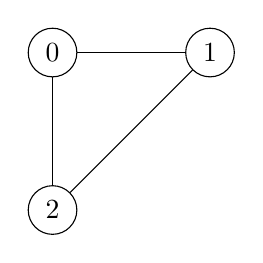
\begin{tikzpicture}
	\node[shape=circle, draw=black] (0) at (0,0)  {0};
	\node[shape=circle, draw=black] (1) at (2,0)  {1};
	\node[shape=circle, draw=black] (2) at (0,-2) {2};

	\path [-] (0) edge (1);
	\path [-] (1) edge (2);
	\path [-] (2) edge (0);
\end{tikzpicture}
\end{center}
\caption{Grafo sin vértices de grado impar inicial}
\end{figure}

El algoritmo empieza en el vértice $v_0$, a partir del cual busca en todos los vértices adyacentes una arista que no sea un puente mediante una búsqueda en profundidad:

\begin{figure}[h]
\begin{center}
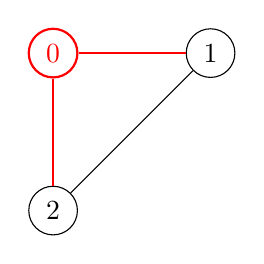
\begin{tikzpicture}
	\node[shape=circle, draw=red, text=red, thick]  (0) at (0,0)  {0};
	\node[shape=circle, draw=black]                 (1) at (2,0)  {1};
	\node[shape=circle, draw=black]                 (2) at (0,-2) {2};

	\path [-, red, thick] (0) edge (1);
	\path [-]             (1) edge (2);
	\path [-, red, thick] (2) edge (0);
\end{tikzpicture}
\end{center}
\caption{Primer vértice seleccionado}
\end{figure}

\pagebreak

Tras esto, realiza una búsqueda en profundidad a partir de cada uno de los vértices en orden cardinal para comprobar si son puentes y proceder con la arista que los une.
En este caso, el algoritmo se posiciona en $v_1$ y realiza una búsqueda en profundidad sin modificar el grafo y eliminando la arista que une $v_1$ y $v_0$:

\begin{figure}[h]
\begin{center}
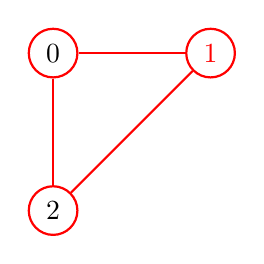
\begin{tikzpicture}
	\node[shape=circle, draw=red, thick]           (0) at (0,0)  {0};
	\node[shape=circle, draw=red, text=red, thick] (1) at (2,0)  {1};
	\node[shape=circle, draw=red, thick]           (2) at (0,-2) {2};

	\path [-, red, thick] (0) edge (1);
	\path [-, red, thick] (1) edge (2);
	\path [-, red, thick] (2) edge (0);
\end{tikzpicture}
\hspace{10mm}
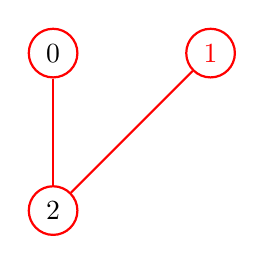
\begin{tikzpicture}
	\node[shape=circle, draw=red, thick]           (0) at (0,0)  {0};
	\node[shape=circle, draw=red, text=red, thick] (1) at (2,0)  {1};
	\node[shape=circle, draw=red, thick]           (2) at (0,-2) {2};

	\path [-, red, thick] (1) edge (2);
	\path [-, red, thick] (2) edge (0);
\end{tikzpicture}
\end{center}
\caption{Búsqueda en profundidad a partir de $v_1$}
\end{figure}

Como el número de vértices accesibles a partir de $v_1$ es igual con la arista que lo une con $v_0$ que sin ella, confirmamos que este nodo no es un puente y procedemos a eliminar la arista $v_0v_1$.

\begin{figure}[h]
\begin{center}
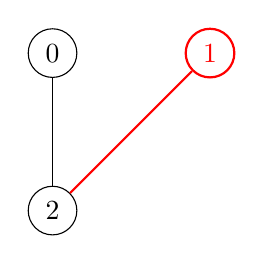
\begin{tikzpicture}
	\node[shape=circle, draw=black]                (0) at (0,0)  {0};
	\node[shape=circle, draw=red, text=red, thick] (1) at (2,0)  {1};
	\node[shape=circle, draw=black]                (2) at (0,-2) {2};

	\path [-, red, thick] (1) edge (2);
	\path [-]             (2) edge (0);
\end{tikzpicture}
\end{center}
\caption{Eliminación de la arista $v_0v_1$}
\end{figure}

Tras esto, repetimos estos mismos pasos con $v_1$ y $v_2$ hasta completar el circuito $v_0v_1v_2v_0$:

\begin{figure}[!h]
\begin{center}
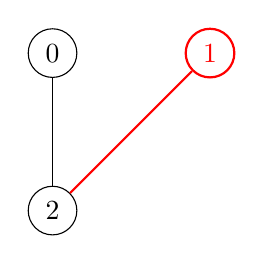
\begin{tikzpicture}
	\node[shape=circle, draw=black]                (0) at (0,0)  {0};
	\node[shape=circle, draw=red, text=red, thick] (1) at (2,0)  {1};
	\node[shape=circle, draw=black]                (2) at (0,-2) {2};

	\path [-, red, thick] (1) edge (2);
	\path [-]             (2) edge (0);
\end{tikzpicture}
\hspace{10mm}
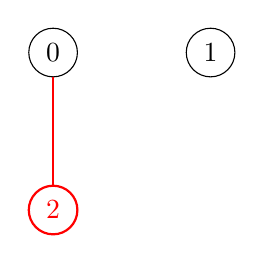
\begin{tikzpicture}
	\node[shape=circle, draw=black]                (0) at (0,0)  {0};
	\node[shape=circle, draw=black]                (1) at (2,0)  {1};
	\node[shape=circle, draw=red, text=red, thick] (2) at (0,-2) {2};

	\path [-, red, thick] (2) edge (0);
\end{tikzpicture}
\hspace{10mm}
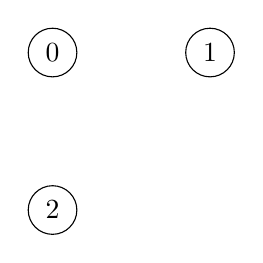
\begin{tikzpicture}
	\node[shape=circle, draw=black]                (0) at (0,0)  {0};
	\node[shape=circle, draw=black]                (1) at (2,0)  {1};
	\node[shape=circle, draw=black]                (2) at (0,-2) {2};
\end{tikzpicture}
\end{center}
\caption{Resto de iteraciones del algoritmo de Fleury para un circuito de Euler}
\end{figure}

\pagebreak

\subsection{Grafo con un camino de Euler}\label{voraces-ejecucion-camino}

Para que el algoritmo ofrezca únicamente un camino de Euler y no un circuito de Euler sobre un grafo, éste debe tener exactamente dos vértices de grado impar.
En este caso, formaremos un grafo de cinco vértices en el que los vértices $v_0$ y $v_1$ son de grado impar.

\begin{figure}[h]
\begin{center}
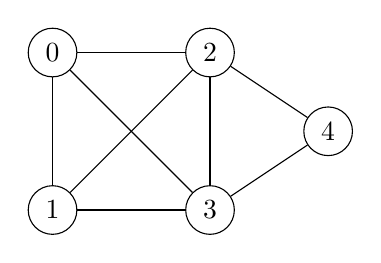
\begin{tikzpicture}
	\node[shape=circle, draw=black] (0) at (0,0)    {0};
	\node[shape=circle, draw=black] (1) at (0,-2)   {1};
	\node[shape=circle, draw=black] (2) at (2,0)    {2};
	\node[shape=circle, draw=black] (3) at (2,-2)   {3};
	\node[shape=circle, draw=black] (4) at (3.5,-1) {4};

	\path [-] (0) edge (1);
	\path [-] (0) edge (2);
	\path [-] (0) edge (3);
	\path [-] (1) edge (2);
	\path [-] (1) edge (3);
	\path [-] (2) edge (3);
	\path [-] (2) edge (4);
	\path [-] (3) edge (4);
\end{tikzpicture}
\end{center}
\caption{Grafo con dos vértices de grado impar inicial}
\end{figure}

Nuestro algoritmo selecciona $v_1$ como vértice inicial y realiza una búsqueda en profundidad para encontrar el siguiente nodo.

\begin{figure}[h]
\begin{center}
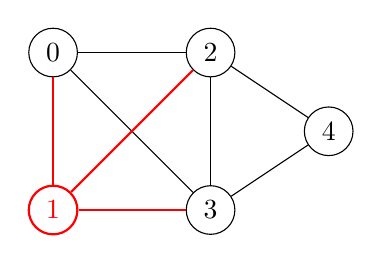
\begin{tikzpicture}
	\node[shape=circle, draw=black]                 (0) at (0,0)    {0};
	\node[shape=circle, draw=red, text=red, thick]  (1) at (0,-2)   {1};
	\node[shape=circle, draw=black]                 (2) at (2,0)    {2};
	\node[shape=circle, draw=black]                 (3) at (2,-2)   {3};
	\node[shape=circle, draw=black]                 (4) at (3.5,-1) {4};

	\path [-, red, thick] (0) edge (1);
	\path [-]             (0) edge (2);
	\path [-]             (0) edge (3);
	\path [-, red, thick] (1) edge (2);
	\path [-, red, thick] (1) edge (3);
	\path [-]             (2) edge (3);
	\path [-]             (2) edge (4);
	\path [-]             (3) edge (4);
\end{tikzpicture}
\end{center}
\caption{Primera iteración del algoritmo de Fleury para un camino de Euler}
\end{figure}

El resto del algoritmo se ejecuta de forma análoga al caso del circuito.

\begin{figure}[!h]
\begin{center}
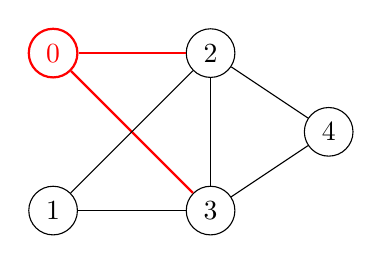
\begin{tikzpicture}
	\node[shape=circle, draw=red, text=red, thick]  (0) at (0,0)    {0};
	\node[shape=circle, draw=black]                 (1) at (0,-2)   {1};
	\node[shape=circle, draw=black]                 (2) at (2,0)    {2};
	\node[shape=circle, draw=black]                 (3) at (2,-2)   {3};
	\node[shape=circle, draw=black]                 (4) at (3.5,-1) {4};

	\path [-, red, thick] (0) edge (2);
	\path [-, red, thick] (0) edge (3);
	\path [-]             (1) edge (2);
	\path [-]             (1) edge (3);
	\path [-]             (2) edge (3);
	\path [-]             (2) edge (4);
	\path [-]             (3) edge (4);
\end{tikzpicture}
\hspace{10mm}
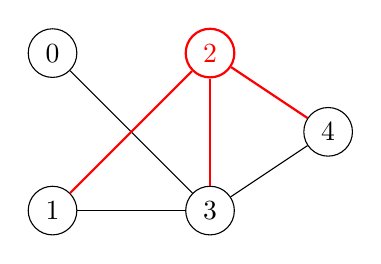
\begin{tikzpicture}
	\node[shape=circle, draw=black]                 (0) at (0,0)    {0};
	\node[shape=circle, draw=black]                 (1) at (0,-2)   {1};
	\node[shape=circle, draw=red, text=red, thick]  (2) at (2,0)    {2};
	\node[shape=circle, draw=black]                 (3) at (2,-2)   {3};
	\node[shape=circle, draw=black]                 (4) at (3.5,-1) {4};

	\path [-]             (0) edge (3);
	\path [-, red, thick] (1) edge (2);
	\path [-]             (1) edge (3);
	\path [-, red, thick] (2) edge (3);
	\path [-, red, thick] (2) edge (4);
	\path [-]             (3) edge (4);
\end{tikzpicture}
\hspace{10mm}
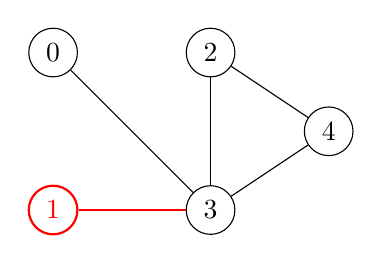
\begin{tikzpicture}
	\node[shape=circle, draw=black]                 (0) at (0,0)    {0};
	\node[shape=circle, draw=red, text=red, thick]  (1) at (0,-2)   {1};
	\node[shape=circle, draw=black]                 (2) at (2,0)    {2};
	\node[shape=circle, draw=black]                 (3) at (2,-2)   {3};
	\node[shape=circle, draw=black]                 (4) at (3.5,-1) {4};

	\path [-]             (0) edge (3);
	\path [-, red, thick] (1) edge (3);
	\path [-]             (2) edge (3);
	\path [-]             (2) edge (4);
	\path [-]             (3) edge (4);
\end{tikzpicture}

\vspace{10mm}

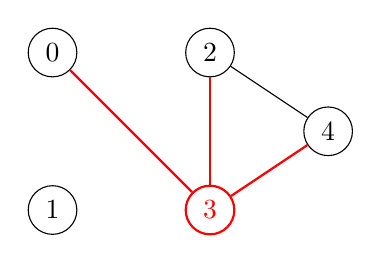
\begin{tikzpicture}
	\node[shape=circle, draw=black]                 (0) at (0,0)    {0};
	\node[shape=circle, draw=black]                 (1) at (0,-2)   {1};
	\node[shape=circle, draw=black]                 (2) at (2,0)    {2};
	\node[shape=circle, draw=red, text=red, thick]  (3) at (2,-2)   {3};
	\node[shape=circle, draw=black]                 (4) at (3.5,-1) {4};

	\path [-, red, thick] (0) edge (3);
	\path [-, red, thick] (2) edge (3);
	\path [-]             (2) edge (4);
	\path [-, red, thick] (3) edge (4);
\end{tikzpicture}
\hspace{10mm}
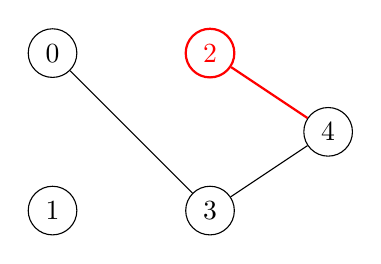
\begin{tikzpicture}
	\node[shape=circle, draw=black]                 (0) at (0,0)    {0};
	\node[shape=circle, draw=black]                 (1) at (0,-2)   {1};
	\node[shape=circle, draw=red, text=red, thick]  (2) at (2,0)    {2};
	\node[shape=circle, draw=black]                 (3) at (2,-2)   {3};
	\node[shape=circle, draw=black]                 (4) at (3.5,-1) {4};

	\path [-]             (0) edge (3);
	\path [-, red, thick] (2) edge (4);
	\path [-]             (3) edge (4);
\end{tikzpicture}
\hspace{10mm}
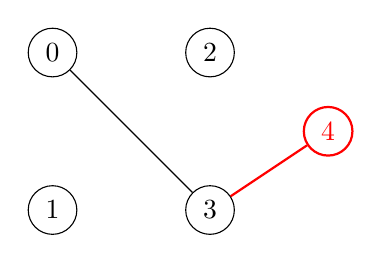
\begin{tikzpicture}
	\node[shape=circle, draw=black]                 (0) at (0,0)    {0};
	\node[shape=circle, draw=black]                 (1) at (0,-2)   {1};
	\node[shape=circle, draw=black]                 (2) at (2,0)    {2};
	\node[shape=circle, draw=black]                 (3) at (2,-2)   {3};
	\node[shape=circle, draw=red, text=red, thick]  (4) at (3.5,-1) {4};

	\path [-]             (0) edge (3);
	\path [-, red, thick] (3) edge (4);
\end{tikzpicture}

\vspace{10mm}

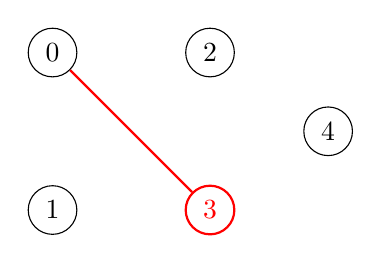
\begin{tikzpicture}
	\node[shape=circle, draw=black]                 (0) at (0,0)    {0};
	\node[shape=circle, draw=black]                 (1) at (0,-2)   {1};
	\node[shape=circle, draw=black]                 (2) at (2,0)    {2};
	\node[shape=circle, draw=red, text=red, thick]  (3) at (2,-2)   {3};
	\node[shape=circle, draw=black]                 (4) at (3.5,-1) {4};

	\path [-, red, thick] (0) edge (3);
\end{tikzpicture}
\hspace{10mm}
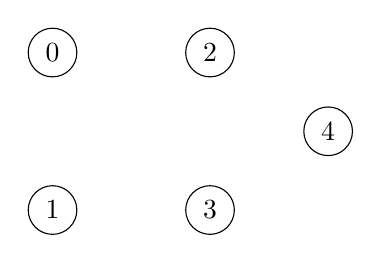
\begin{tikzpicture}
	\node[shape=circle, draw=black] (0) at (0,0)    {0};
	\node[shape=circle, draw=black] (1) at (0,-2)   {1};
	\node[shape=circle, draw=black] (2) at (2,0)    {2};
	\node[shape=circle, draw=black] (3) at (2,-2)   {3};
	\node[shape=circle, draw=black] (4) at (3.5,-1) {4};
\end{tikzpicture}
\end{center}
\caption{Resto de iteraciones del algoritmo de Fleury para un camino de Euler}
\end{figure}

Al final la ejecución del algoritmo sobr eeste grafo devuelve el camino $v_1v_0v_2v_1v_3v_2v_4v_3v_0$.
